\documentclass[12pt,a4paper,twocolumn]{article}
\usepackage[]{accanthis}
\usepackage{amssymb,amsmath}
\usepackage{ifxetex,ifluatex}
\usepackage{fixltx2e} % provides \textsubscript
\ifnum 0\ifxetex 1\fi\ifluatex 1\fi=0 % if pdftex
  \usepackage[T1]{fontenc}
  \usepackage[utf8]{inputenc}
\else % if luatex or xelatex
  \ifxetex
    \usepackage{mathspec}
  \else
    \usepackage{fontspec}
  \fi
  \defaultfontfeatures{Ligatures=TeX,Scale=MatchLowercase}
\fi
% use upquote if available, for straight quotes in verbatim environments
\IfFileExists{upquote.sty}{\usepackage{upquote}}{}
% use microtype if available
\IfFileExists{microtype.sty}{%
\usepackage[]{microtype}
\UseMicrotypeSet[protrusion]{basicmath} % disable protrusion for tt fonts
}{}
\PassOptionsToPackage{hyphens}{url} % url is loaded by hyperref
\usepackage[unicode=true]{hyperref}
\PassOptionsToPackage{usenames,dvipsnames}{color} % color is loaded by hyperref
\hypersetup{
            pdftitle={Functional Comparisons between Ocean Regions},
            pdfauthor={Dustin Michels},
            colorlinks=true,
            linkcolor=Maroon,
            citecolor=Blue,
            urlcolor=Blue,
            breaklinks=true}
\urlstyle{same}  % don't use monospace font for urls
\usepackage[top=1.5cm, bottom=2.5cm, left=1.5cm, right=1.5cm]{geometry}
\usepackage{graphicx,grffile}
\makeatletter
\def\maxwidth{\ifdim\Gin@nat@width>\linewidth\linewidth\else\Gin@nat@width\fi}
\def\maxheight{\ifdim\Gin@nat@height>\textheight\textheight\else\Gin@nat@height\fi}
\makeatother
% Scale images if necessary, so that they will not overflow the page
% margins by default, and it is still possible to overwrite the defaults
% using explicit options in \includegraphics[width, height, ...]{}
\setkeys{Gin}{width=\maxwidth,height=\maxheight,keepaspectratio}
\setlength{\emergencystretch}{3em}  % prevent overfull lines
\providecommand{\tightlist}{%
  \setlength{\itemsep}{0pt}\setlength{\parskip}{0pt}}
\setcounter{secnumdepth}{0}
% Redefines (sub)paragraphs to behave more like sections
\ifx\paragraph\undefined\else
\let\oldparagraph\paragraph
\renewcommand{\paragraph}[1]{\oldparagraph{#1}\mbox{}}
\fi
\ifx\subparagraph\undefined\else
\let\oldsubparagraph\subparagraph
\renewcommand{\subparagraph}[1]{\oldsubparagraph{#1}\mbox{}}
\fi

% set default figure placement to htbp
\makeatletter
\def\fps@figure{htbp}
\makeatother

% \usepackage[vmargin=1in,hmargin=1in]{geometry}
% \usepackage{lineno}
% \linenumbers
% \usepackage{times}

\title{Functional Comparisons between Ocean Regions}
\author{Dustin Michels}
\date{Nov 2017}

\begin{document}
\maketitle

\listoffigures
\subsection{Abstract}\label{abstract}

No abstract yet\ldots{}

\subsection{Introduction}\label{introduction}

This project is inspired by the paper ``Structure and function of the
global ocean microbiome'' by Sunagawa et al. {[}1{]}, as well as the
paper ``An obesity-associated gut microbiome with increased capacity for
energy harvest'' by Turnbaugh et al. {[}2{]}. The first paper seeks to
characterize staxonomic differences and differences in gene function
between ocean microbiomes, using Tara Ocean samples from around the
world. They seek to identify which factors could best explain that
variation. The second paper, by Turnbaugh et al., at one point describes
the differences between the distal gut microbiomes of mice using
functional annotations of the various microbiomes, and visualizes the
result using heat maps.

My goal in this paper was to employ some of the tactics of the Turnbaugh
et al paper-- understanding the functional differences between
metagenomes using heat maps-- to the domain of the Sunagawa et al.
paper, characterizing functional differences between ocean regions.

One thing to note: I am interested in the challenge of ensuring
reproducibility in bioinformatics projects, and have attempted to
structure this investigation for maximum reproducibility. Namely,

\begin{itemize}
\tightlist
\item
  All files are being stored (at various stages) using a public GitHub
  repository (See:
  \url{https://github.com/dustinmichels/biol338-final-project/tree/master}).
\item
  I am attempting to carry out most stages of data collection, analysis,
  and presentation, using scripts that should be viable to re-run on
  other machines at other times to generate the same results. Even this
  report is being written in plain-text (Markdown) and converted into a
  report using a tool called Pandoc!
\item
  Finally, I am taking care to document the software I am using, and
  which version I am using, and how I am using it.
\end{itemize}

\subsection{Methods}\label{methods}

I have used the eleven Tara Ocean samples that our class has used
throughout the term, but I have downloaded Gene Ontology (GO) files for
each dataset, which detail the number of reads from that dataset that
mapped to each of about 2000 different functional categories, pertaining
to molecular function, cellular components, or biological processes.

For each dataset, I normalized the `read count' into a `read proportion'
(the number of reads that mapped to a given functional category out of
all the reads.) I then selected the top 30 most abundant functional
categories, for each dataset. I ended up dropping three of these
functional categories from my analysis, which had missing data for one
or more samples. That is to say, I wound up plotting the \emph{union} of
the 30 most abundant functional groups from each sample, which is 27
functional groups.

I created three heat maps, one for all eleven samples, one grouped by
region, and one grouped by zone.

I then created three ``cluster maps.'' A cluster map is similar to a
heat map, except it clusters data hierarchically. It calculates pairwise
Euclidean distance between observations in n-dimensional space, and
groups closely related attributes together. It rearranges data
accordingly, and even draws tree structures resembling phylogenies to
indicate groupings. This method produced pretty interesting results, but
I will need to further investigate exactly how this works to ensure the
results are meaningful.

The exact steps I took to do this analysis can be seen and reproduced
online at \url{http://bit.ly/2zEMitP}.

\subsection{Results}\label{results}

Here are the heat maps and cluster maps that I generated.

\begin{figure}
\centering
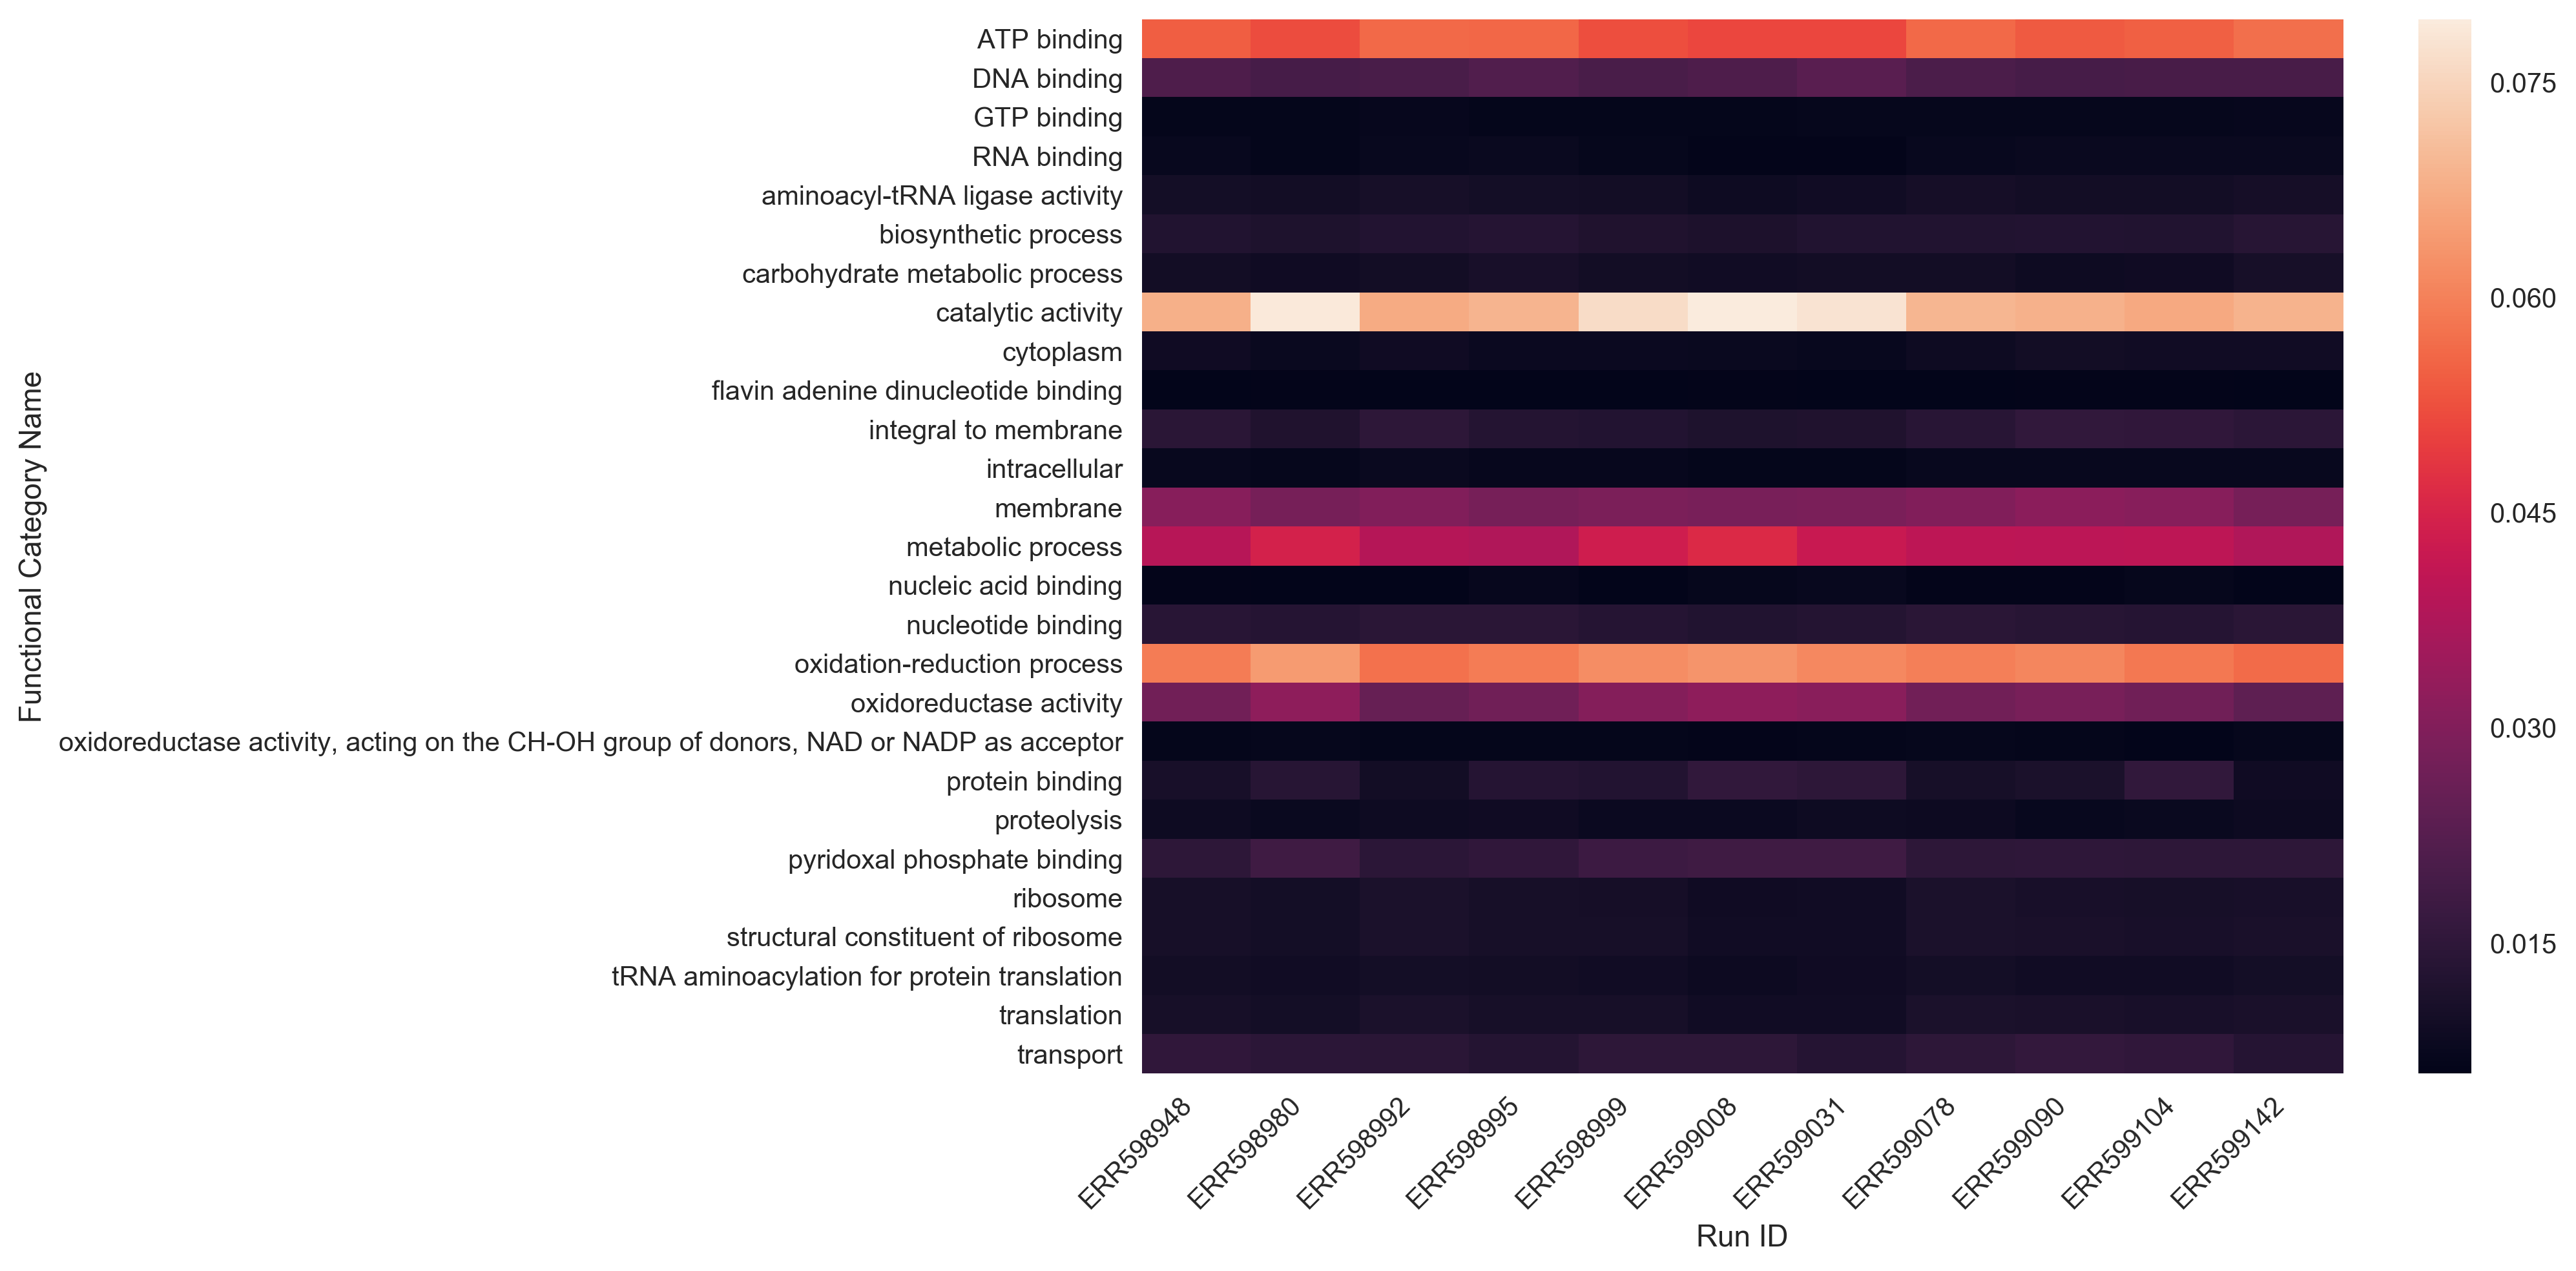
\includegraphics{imgs/heat/heat_all.png}
\caption{Heat map for all samples\label{fig:heat_all}}
\end{figure}

\begin{figure}
\centering
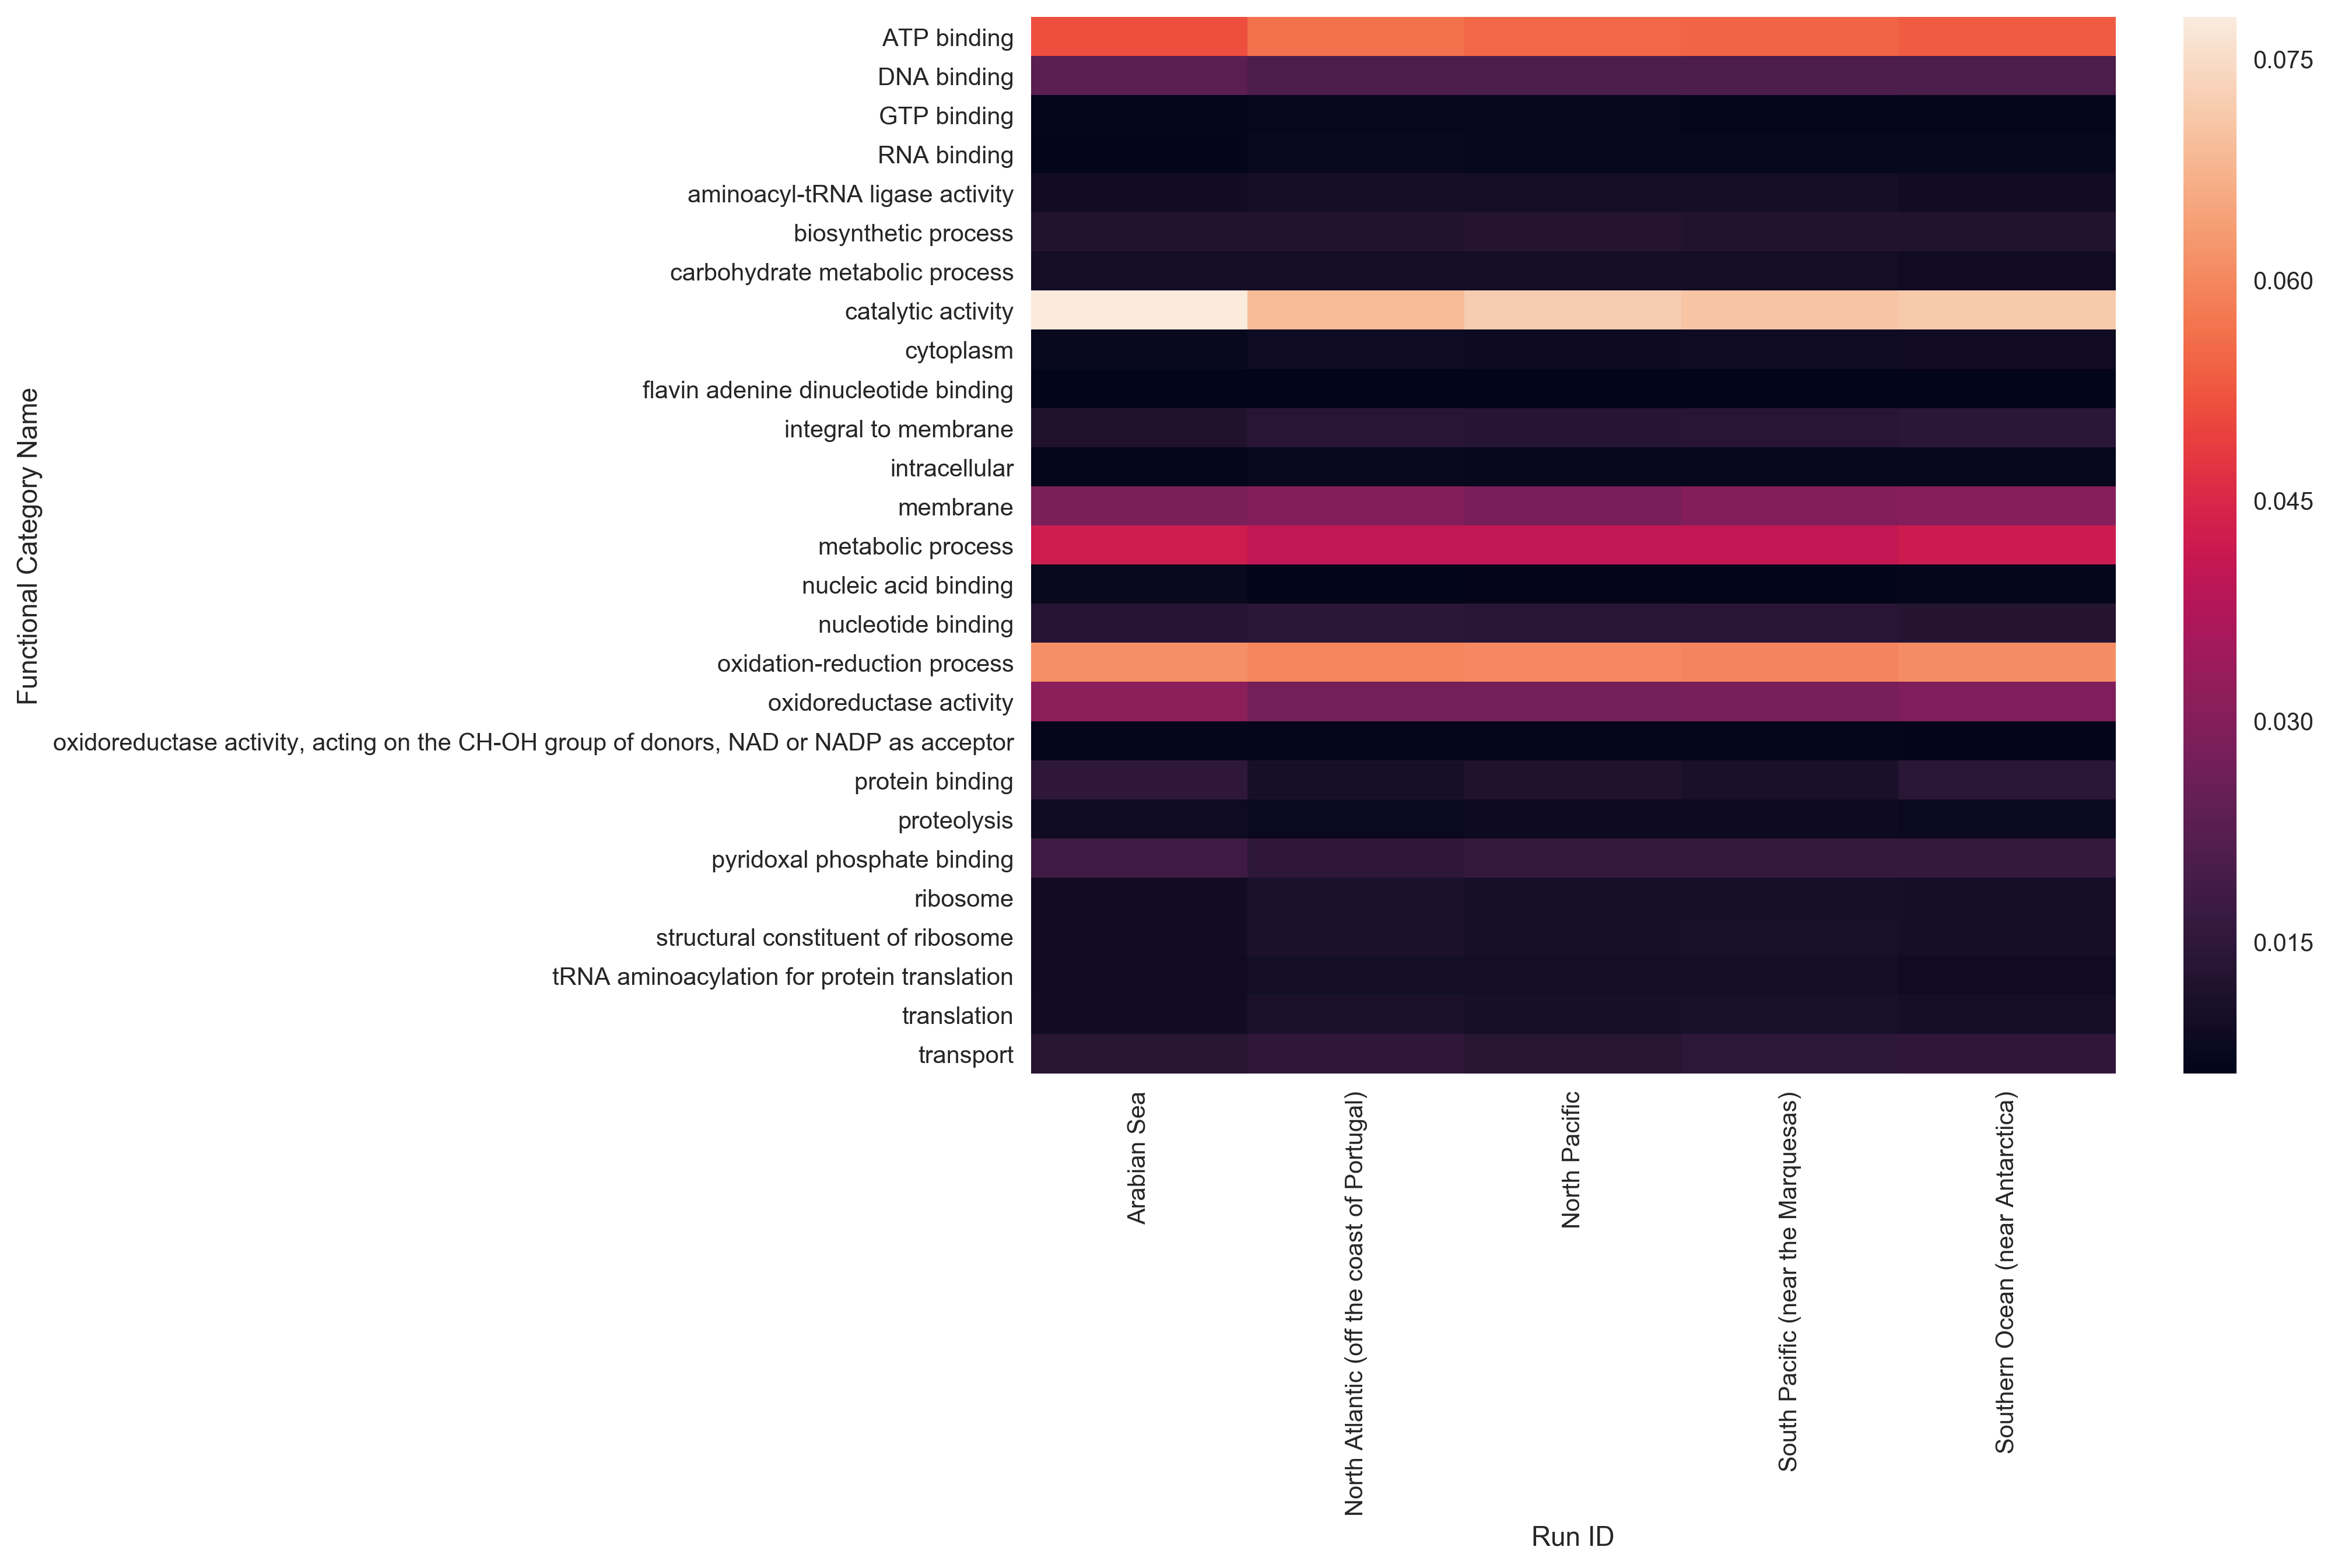
\includegraphics{imgs/heat/heat_region.png}
\caption{Heat map, grouped by region\label{fig:heat_region}}
\end{figure}

\begin{figure}
\centering
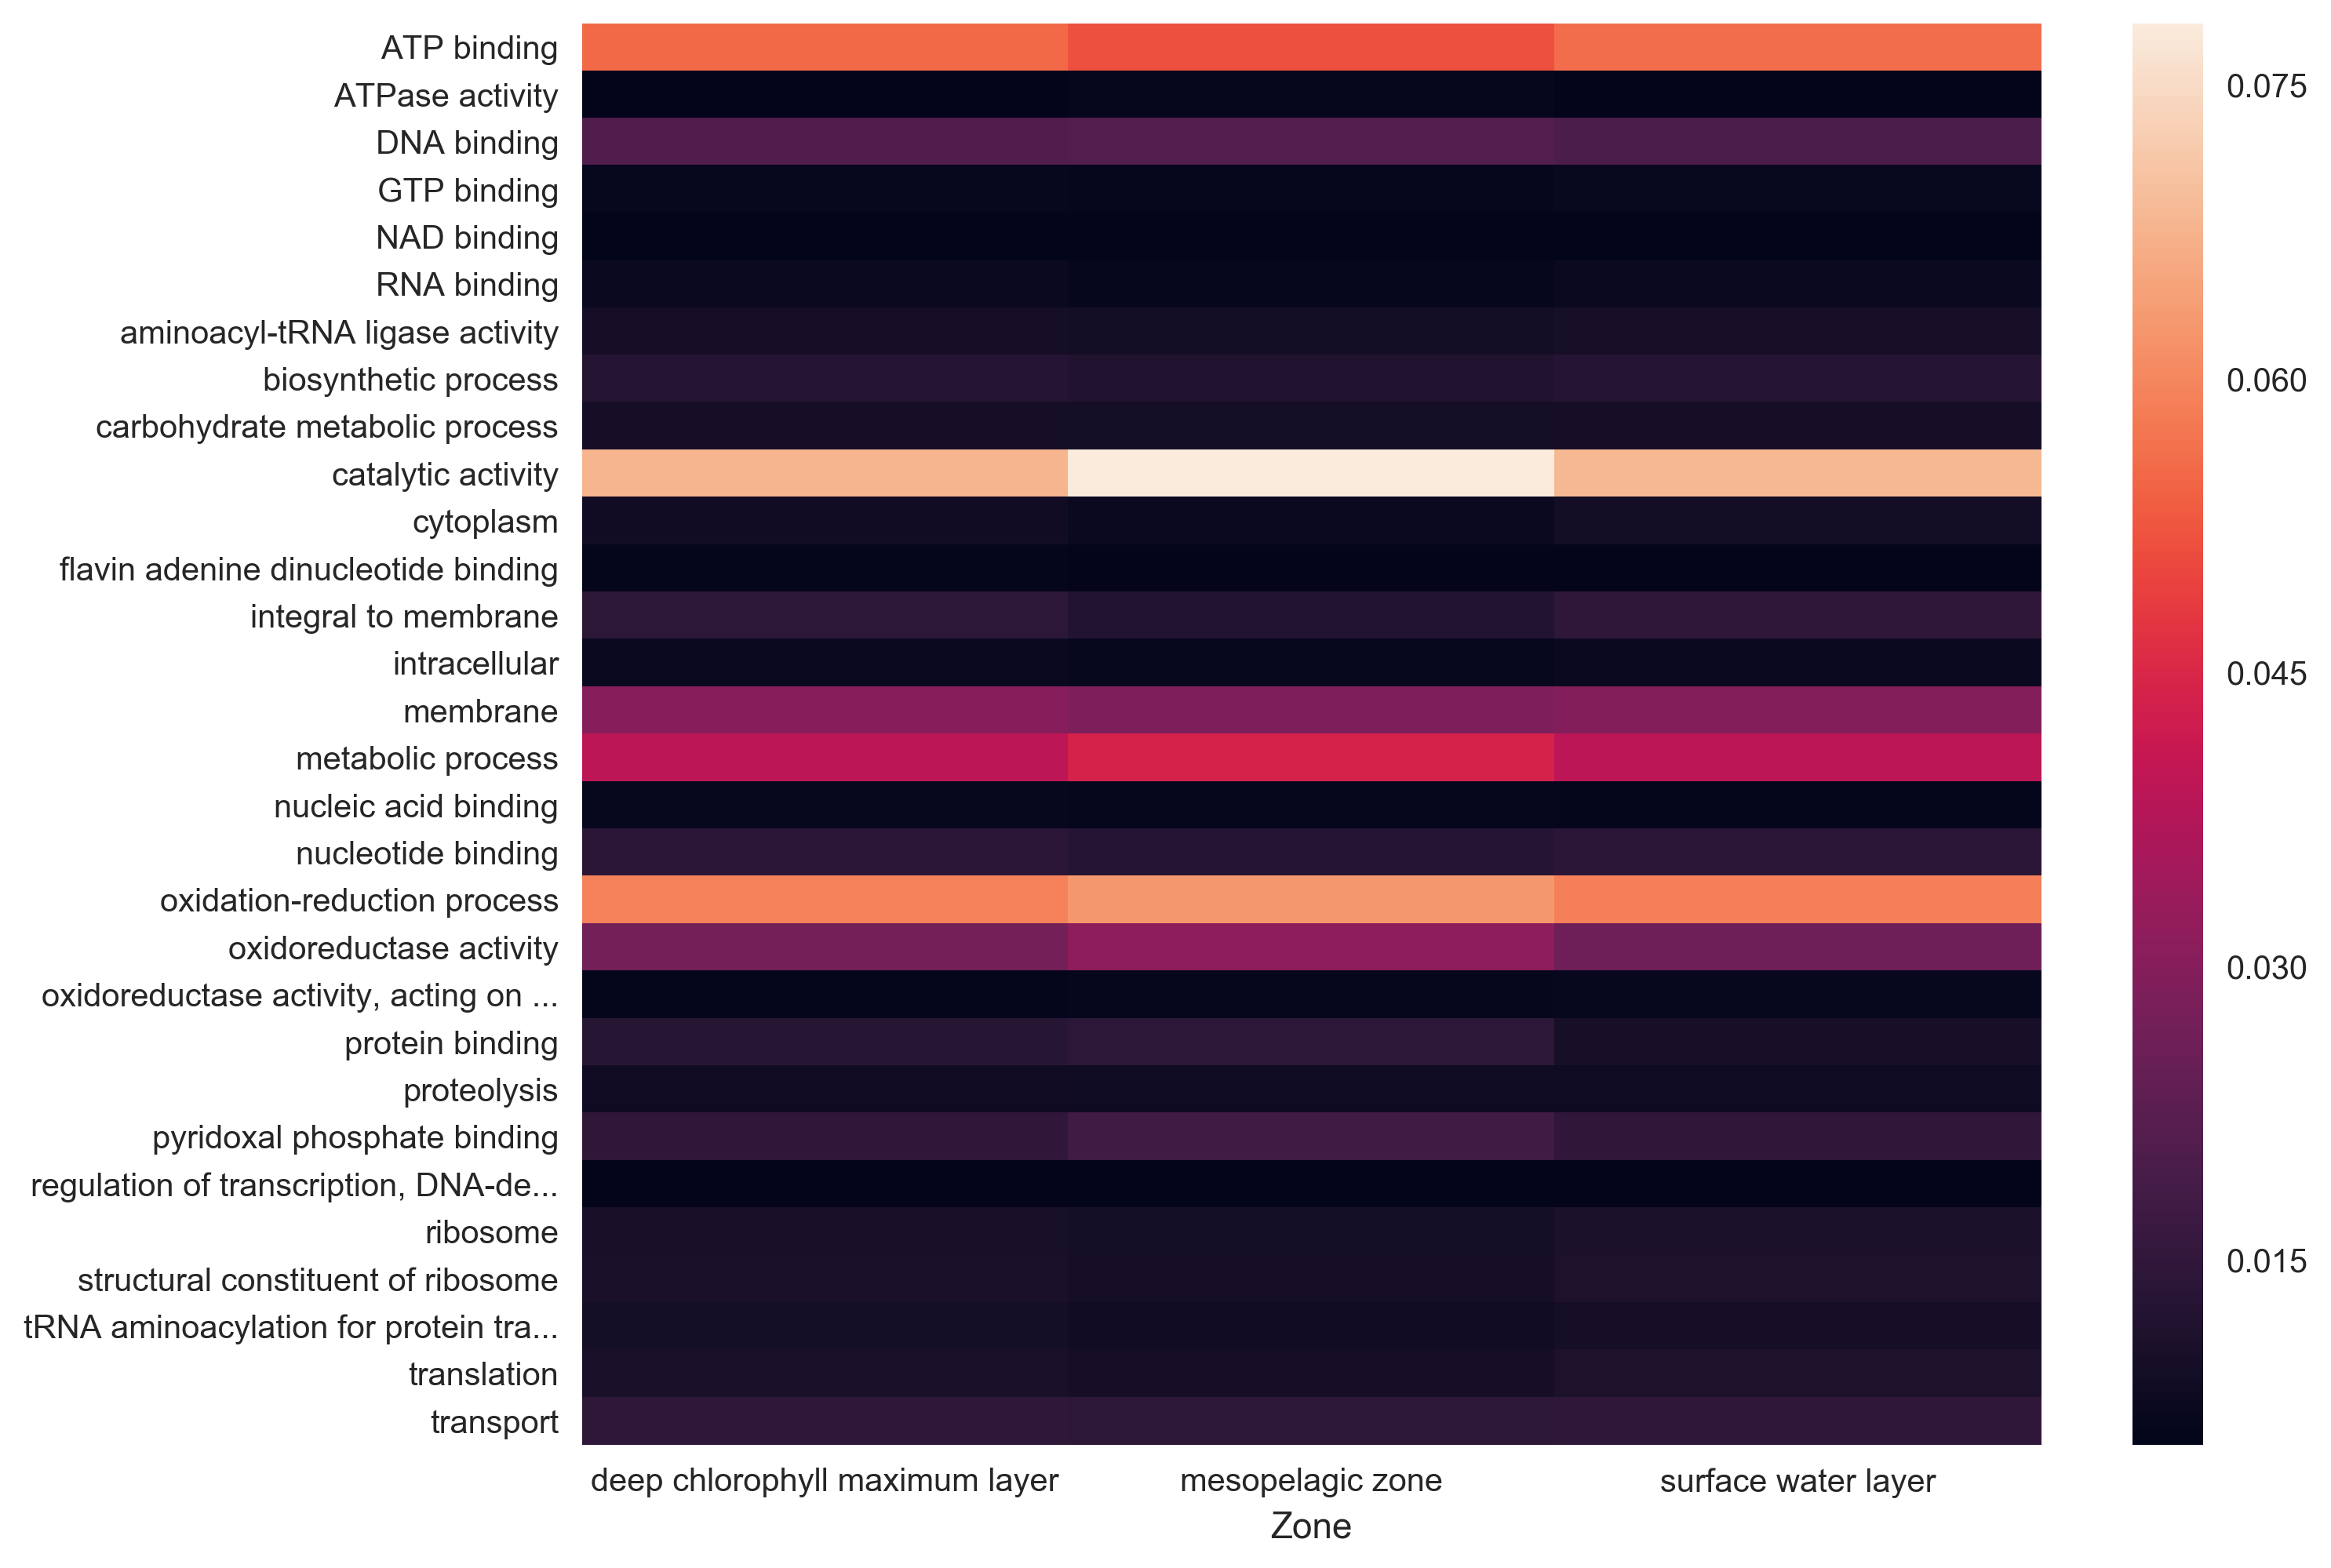
\includegraphics{imgs/heat/heat_zone.png}
\caption{Heat map, grouped by zone\label{fig:heat_zone}}
\end{figure}

\begin{figure}
\centering
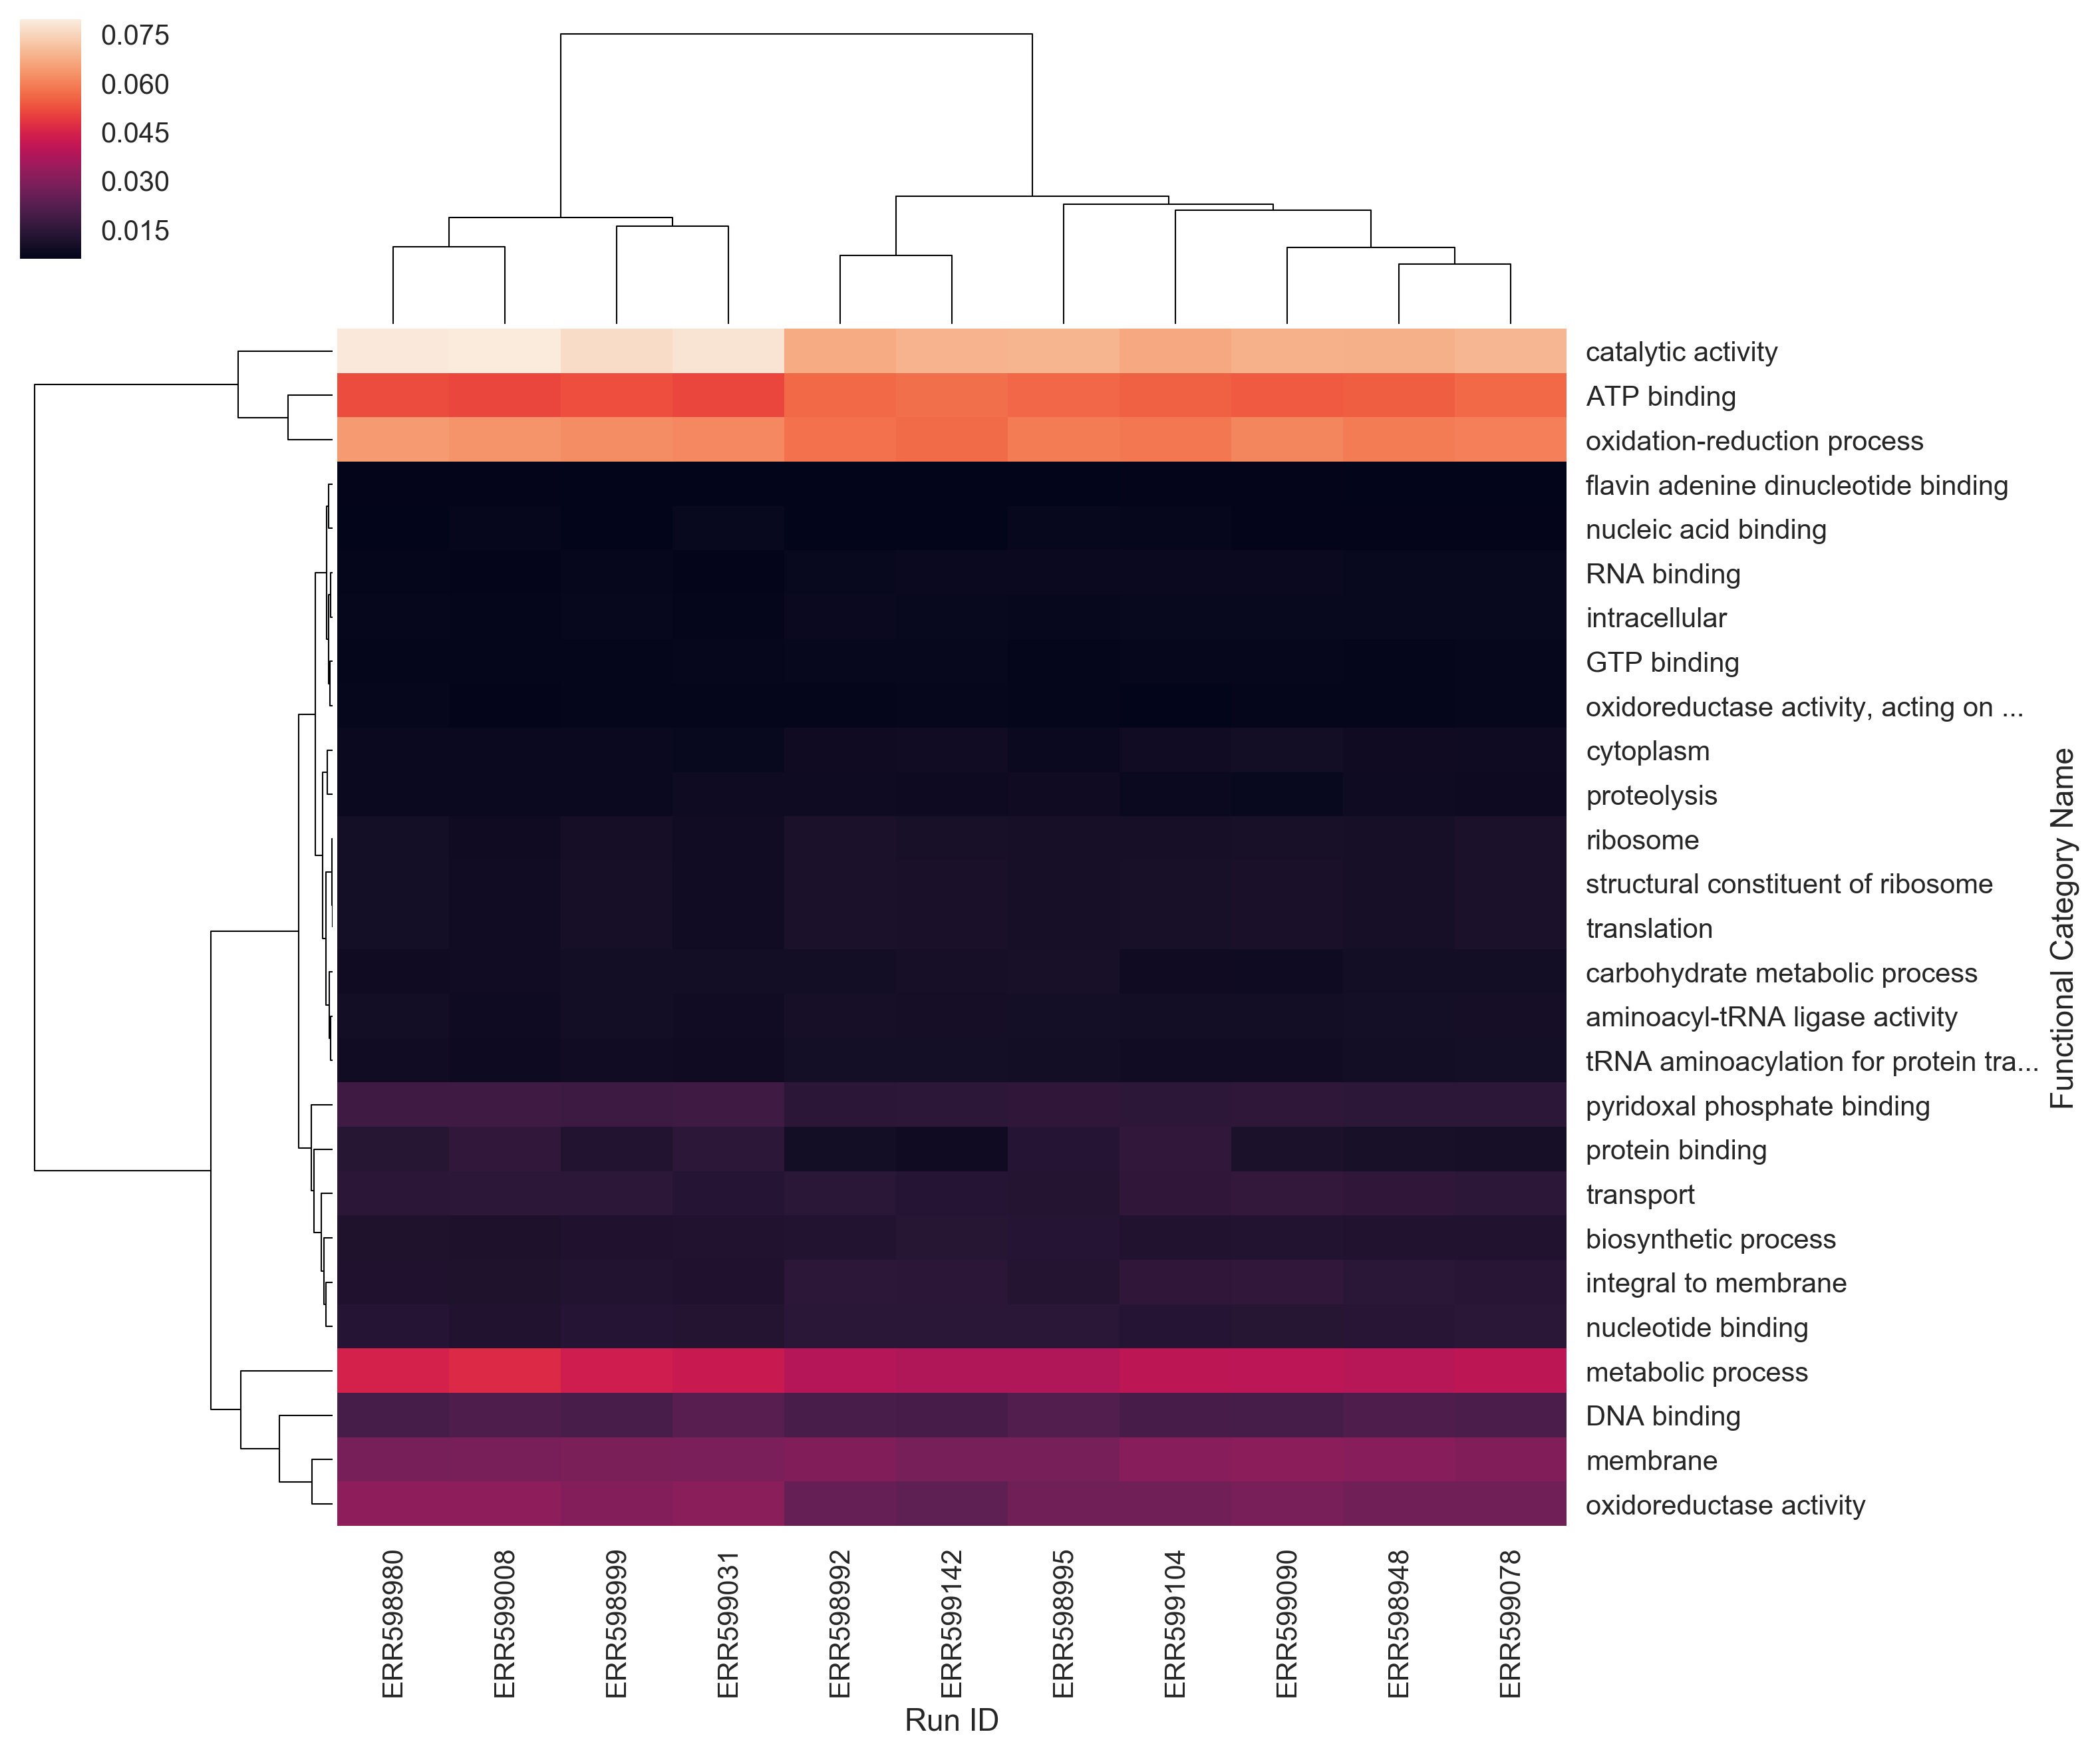
\includegraphics{imgs/cluster/cluster_all.png}
\caption{Cluster map for all samples\label{fig:cluster_all}}
\end{figure}

\begin{figure}
\centering
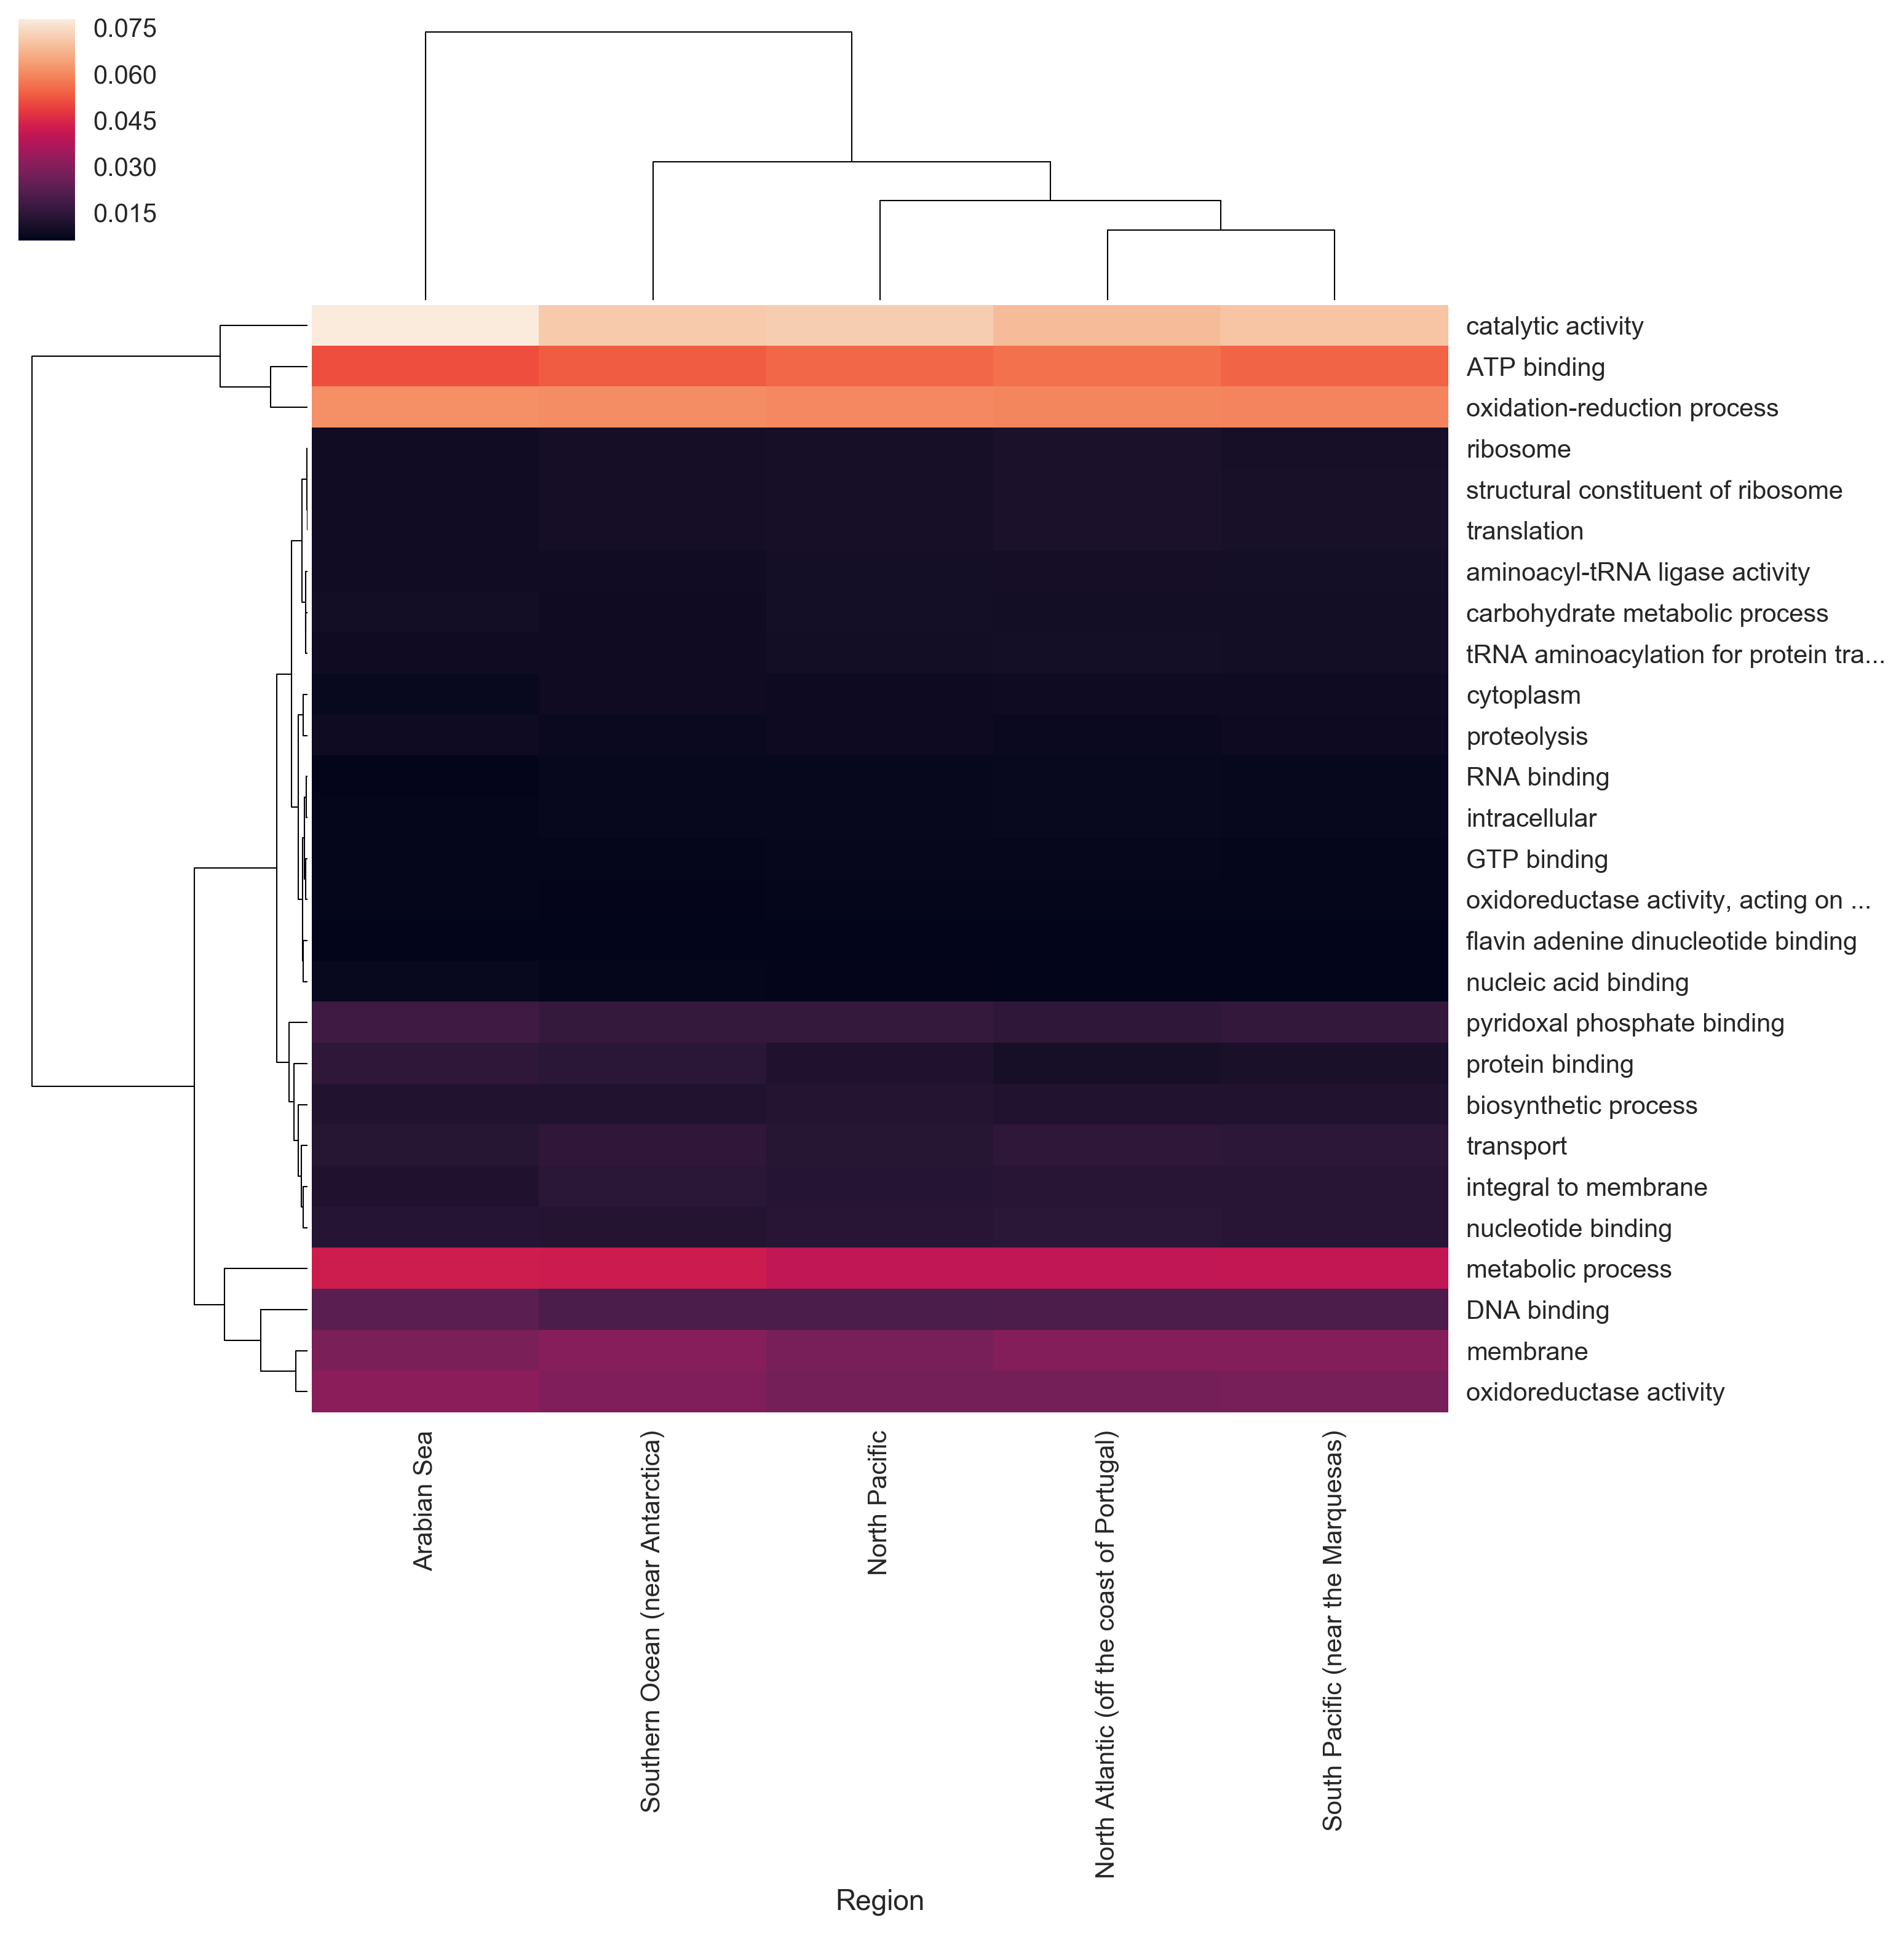
\includegraphics{imgs/cluster/cluster_region.png}
\caption{Cluster map, grouped by region\label{fig:cluster_region}}
\end{figure}

\begin{figure}
\centering
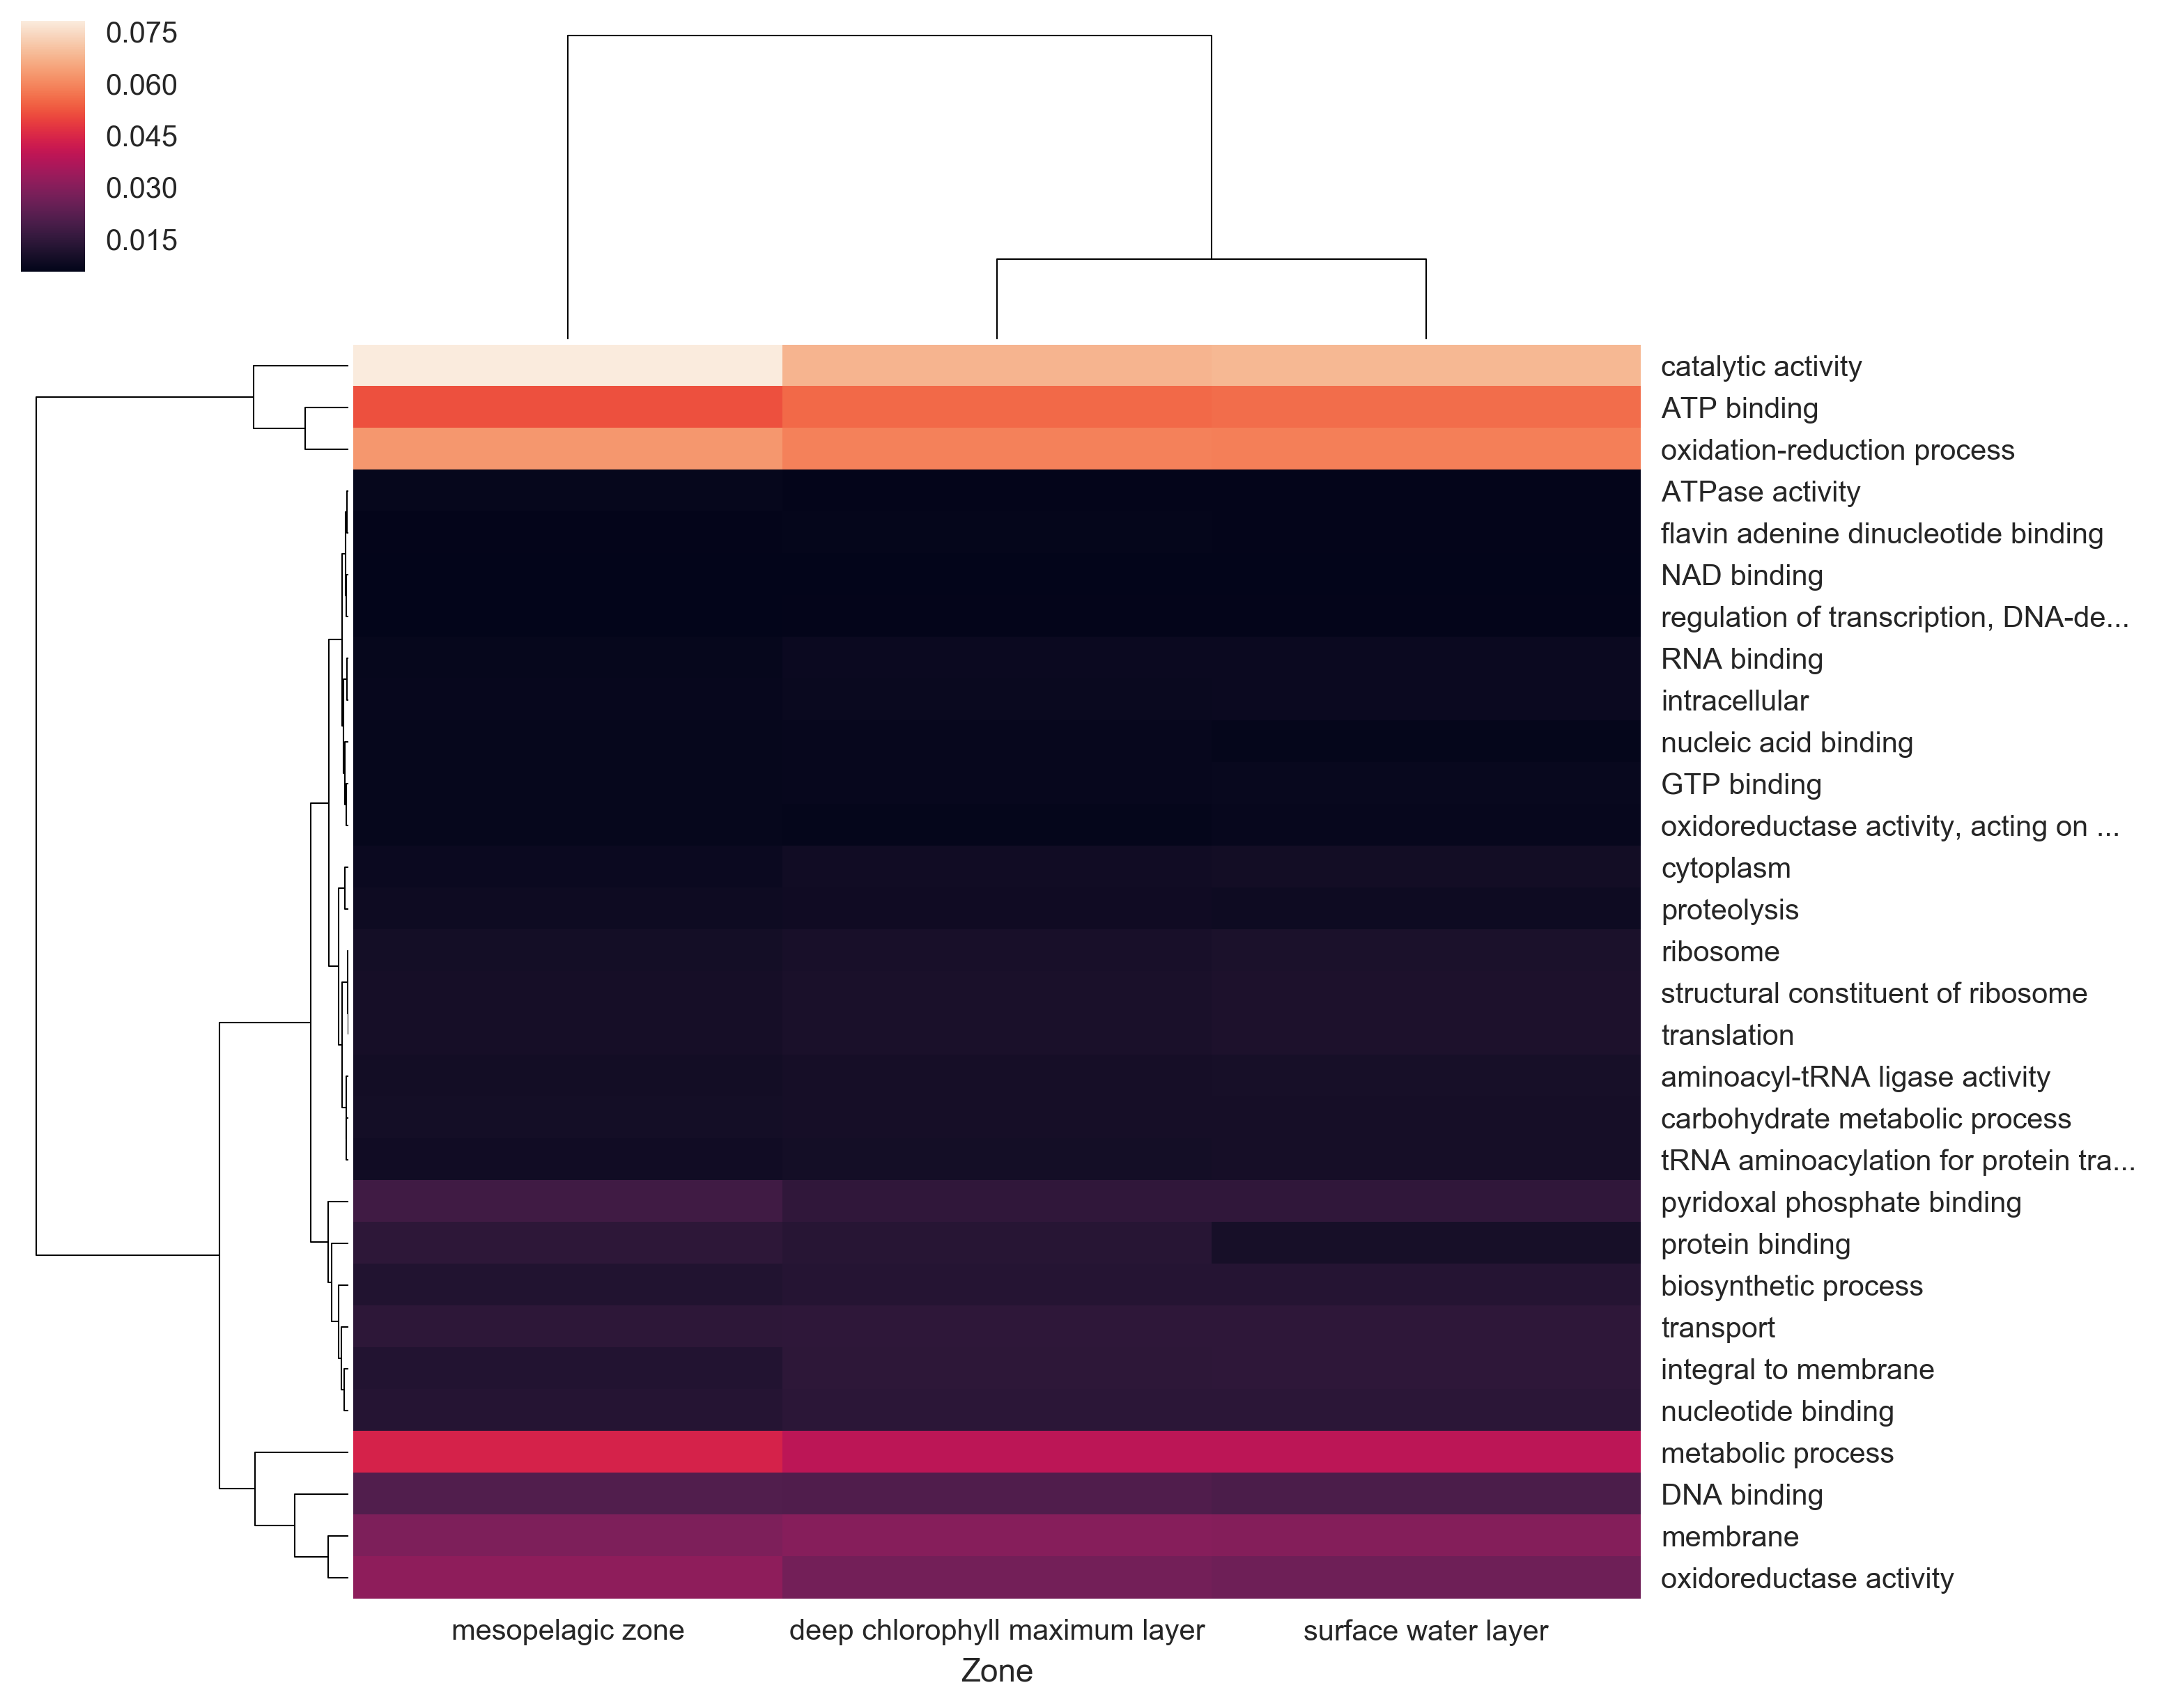
\includegraphics{imgs/cluster/cluster_zone.png}
\caption{Cluster map, grouped by zone\label{fig:cluster_zone}}
\end{figure}

\subsection{Discussion}\label{discussion}

The cluster maps seem to suggest that deep chlorophyll maximum layer and
the surface water later are more closely related to each other, in terms
of prevalence of functional gene categories, prevalence than either is
to the mesopelagic zone

Similarly, the cluster maps would suggest that the North Atlantic and
South Atlantic are the most functionally similar, followed by the North
Pacific, followed by the Souther Ocean, and finally the Arabian Sea.

More analysis underway!

\subsection*{References}\label{references}
\addcontentsline{toc}{subsection}{References}

\hypertarget{refs}{}
\hypertarget{ref-sunagawa_structure_2015}{}
1. Sunagawa S, Coelho LP, Chaffron S, Kultima JR, Labadie K, Salazar G,
et al. Structure and function of the global ocean microbiome. Science.
2015;348: 1261359.
doi:\href{https://doi.org/10.1126/science.1261359}{10.1126/science.1261359}

\hypertarget{ref-turnbaugh_obesity-associated_2006}{}
2. Turnbaugh PJ, Ley RE, Mahowald MA, Magrini V, Mardis ER, Gordon JI.
An obesity-associated gut microbiome with increased capacity for energy
harvest. Nature. 2006;444: 1027--131.
doi:\href{https://doi.org/10.1038/nature05414}{10.1038/nature05414}

\end{document}
